\appendix
\section{Transmisjonskurver}

\begin{figure}[H]%
\centering
%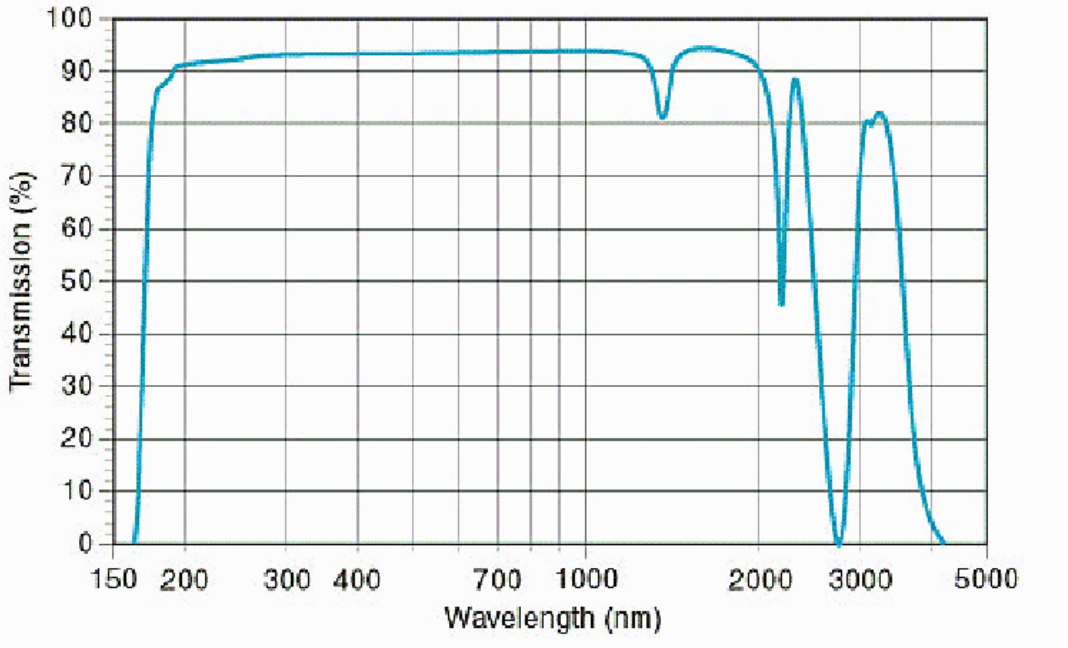
\includegraphics[width=10cm,bb=0 0 1068 648]{cryovindu}%
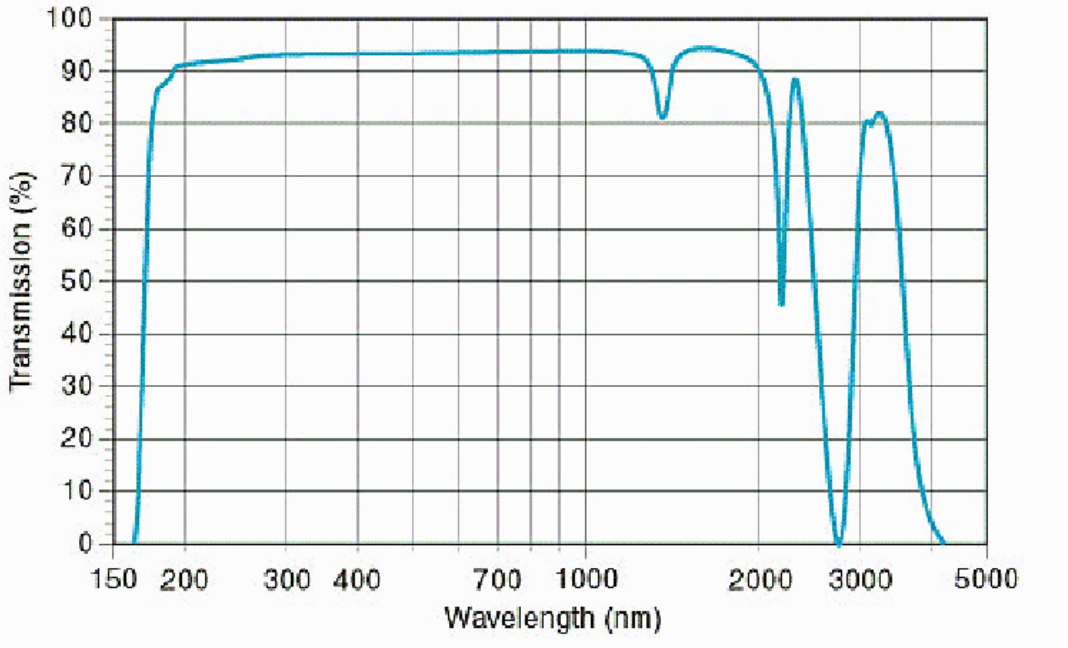
\includegraphics[width=10cm]{cryovindu}%
\caption{Transmisjon gjennom viduet til cryostaten \cite{cryostat} 27.10.2009}%
\label{fig:cryovindu}%
\end{figure}

\begin{figure}[H]%
\centering
%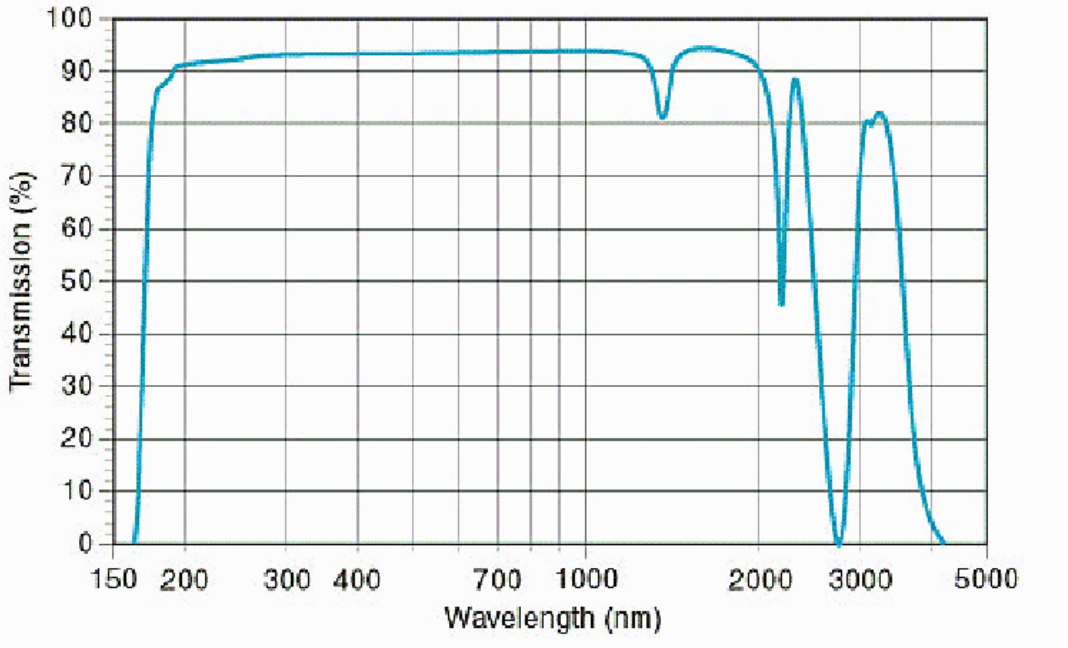
\includegraphics[width=10cm,bb=0 0 1068 648]{cryovindu}%
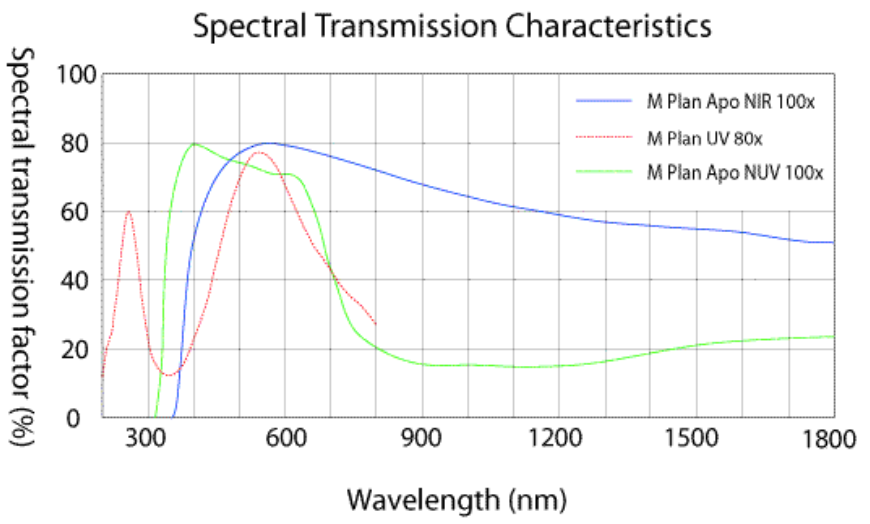
\includegraphics[width=10cm]{objektiv}%
\caption{Transmisjon gjennom objektivet \cite{objektiv} 08.12.2009}%
\label{fig:objektiv}%
\end{figure}

\begin{figure}[H]%
\centering
%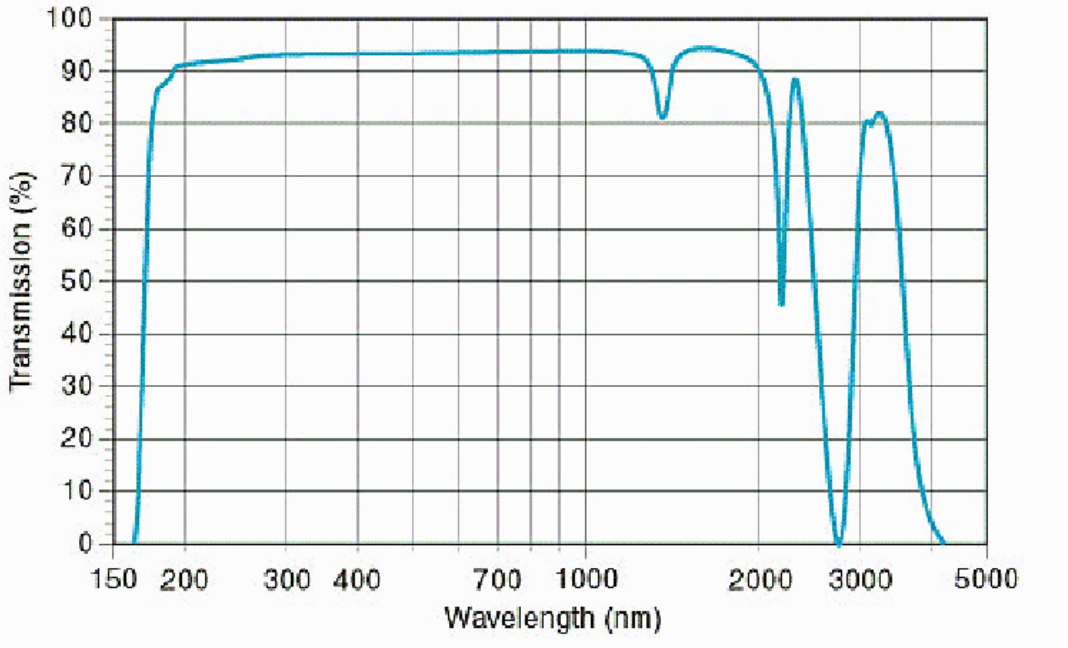
\includegraphics[width=10cm,bb=0 0 1068 648]{cryovindu}%
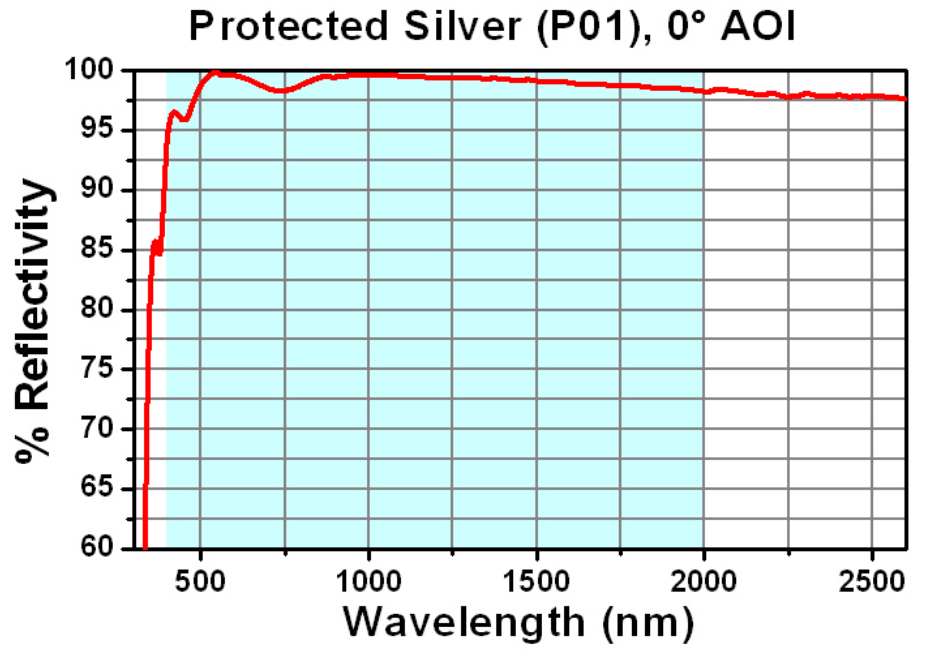
\includegraphics[width=10cm]{speil}%
\caption{Refleksjon for speil \cite{speil} 08.12.2009}%
\label{fig:speil}%
\end{figure}

\begin{figure}[H]%
\centering
%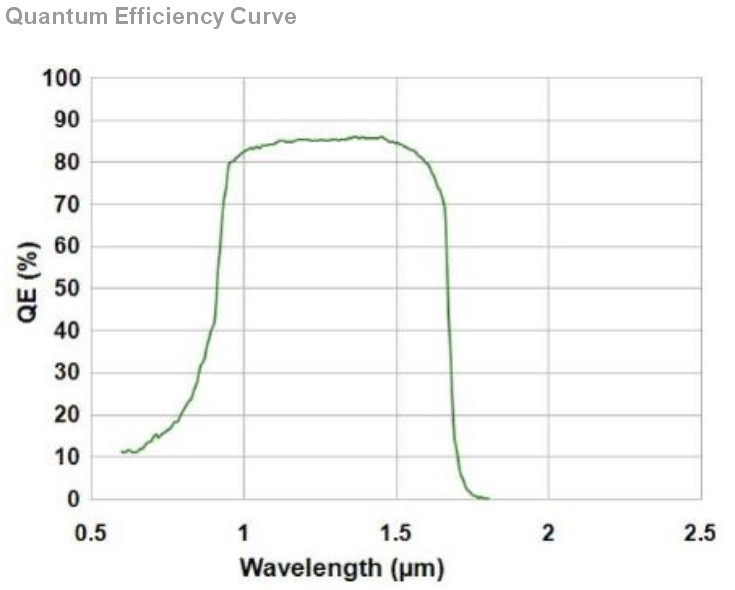
\includegraphics[width=10cm,bb=0 0 735 590]{kameragraf}%
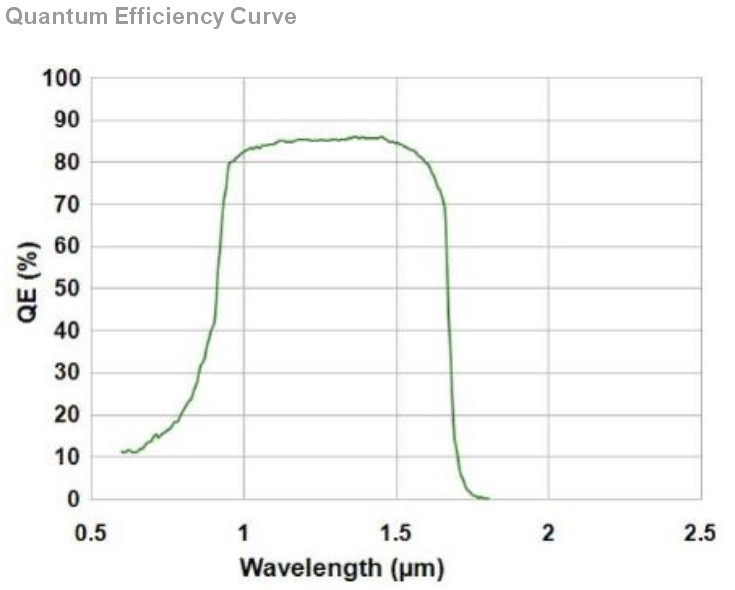
\includegraphics[width=10cm]{kameragraf}%
\caption{Kameraeffektivitet \cite{kamera} 27.10.2009}%
\label{fig:kameragraf}%
\end{figure}



\subsection{F�rste veibane}

\begin{figure}[H]%
\centering
%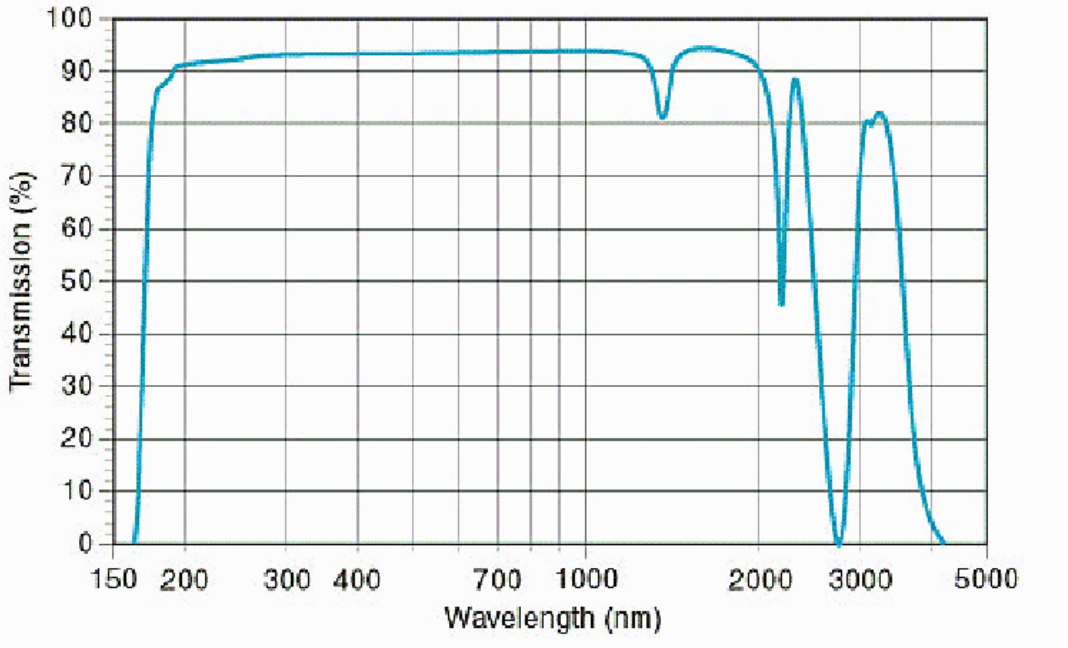
\includegraphics[width=10cm,bb=0 0 1068 648]{cryovindu}%
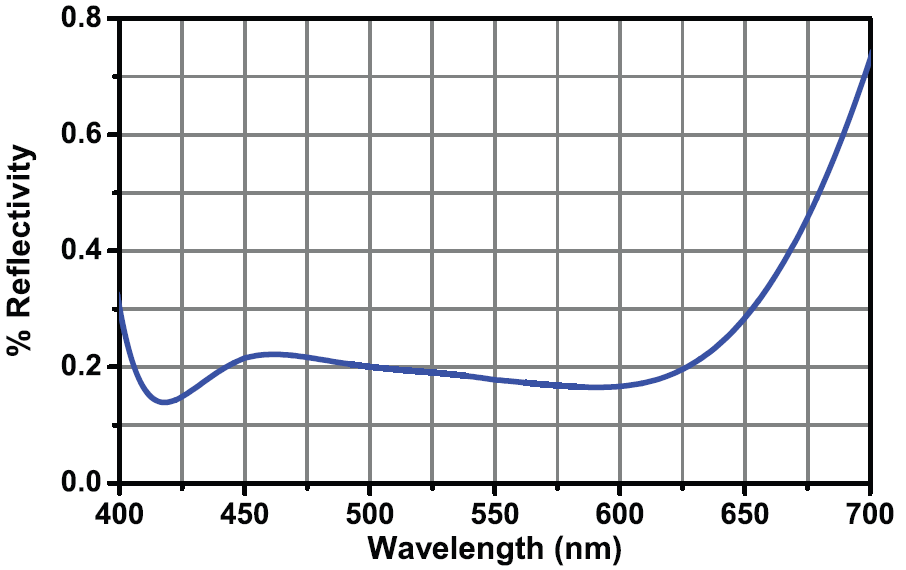
\includegraphics[width=10cm]{breamsplitter400-700nm}%
\caption{Beamsplitter refleksjon fra datablad optimalisert for 400-700nm \cite{beamsplitter} 12.12.2009}%
\label{fig:beamsplitter400-700nm}%
\end{figure}

\begin{figure}[H]%
\centering
%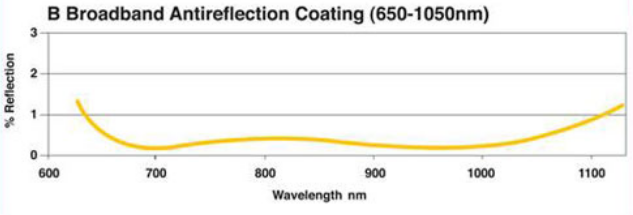
\includegraphics[width=10cm,bb=0 0 633 215]{old_linse}%
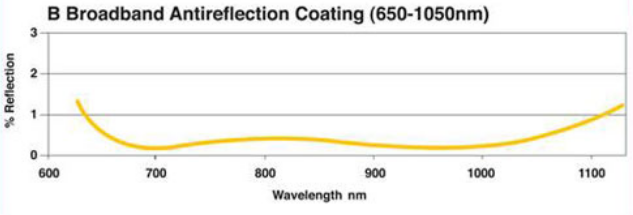
\includegraphics[width=10cm]{old_linse}%
\caption{Transmisjon gjennom linse fra gammel veibane \cite{old_lens} 27.10.2009}%
\label{fig:linsetrans}%
\end{figure}

\subsection{Andre veibane}

\begin{figure}[H]%
\centering
%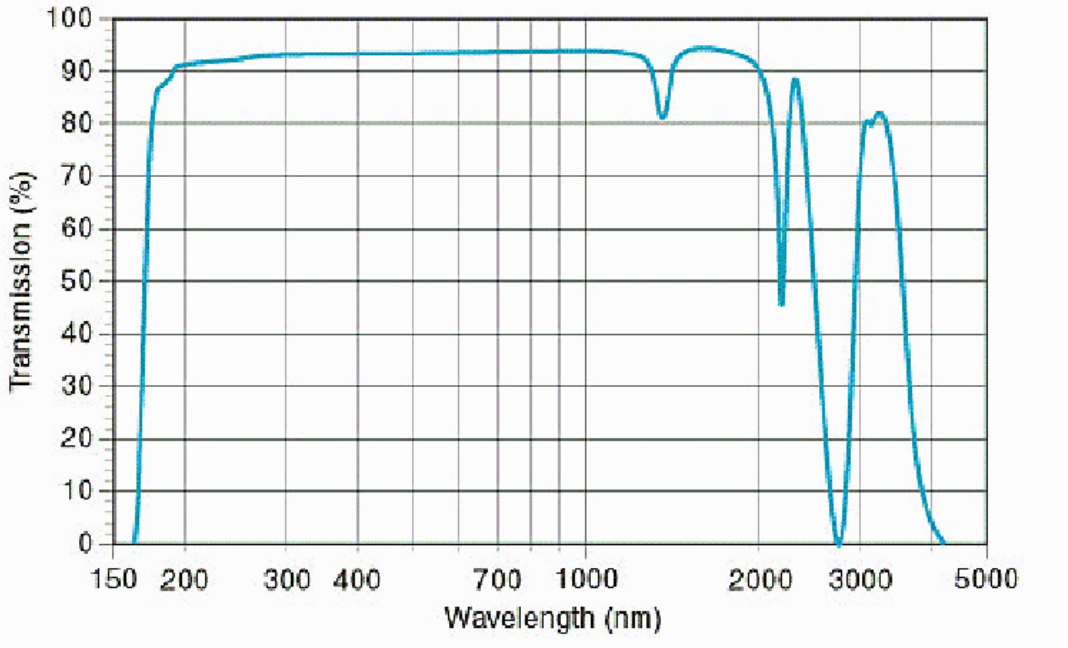
\includegraphics[width=10cm,bb=0 0 1068 648]{cryovindu}%
\includegraphics[width=10cm]{breamsplitter1100-1600nm \cite{beamsplitter_ny} 12.12.2009}%
\caption{Beamsplitter refleksjon fra datablad optimalisert for 1100-1600nm}%
\label{fig:beamsplitter1100-1600nm}%
\end{figure}

\begin{figure}[H]%
\centering
%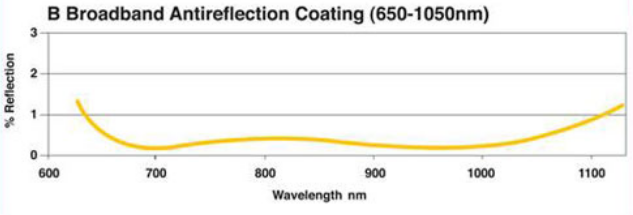
\includegraphics[width=10cm,bb=0 0 633 215]{old_linse}%
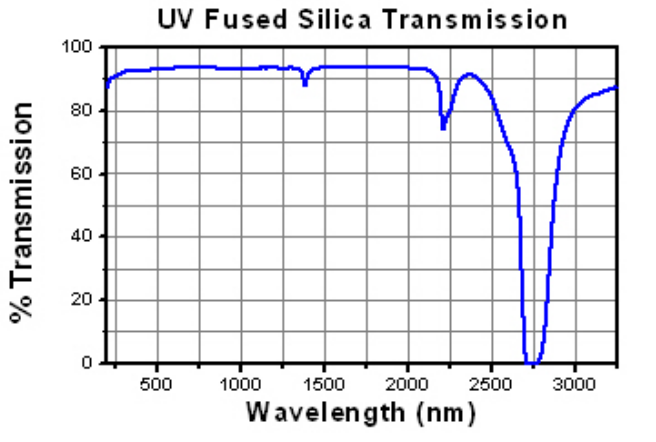
\includegraphics[width=10cm]{ny_linse}%
\caption{Transmisjon gjennom ny linse \cite{new_lens} 08.12.2009}%
\label{fig:linsetrans_ny}%
\end{figure}